\documentclass[twocolumn, 11pt]{article}
\usepackage[a4paper, margin=1in]{geometry}
\usepackage[utf8]{inputenc}
\usepackage{amsmath}
\usepackage{pgfplots}
\usepackage{listings}
\usepackage{xcolor}
\usepackage{graphicx}
\usepgfplotslibrary{groupplots}

\lstset{
  language=C++,
  basicstyle=\ttfamily\small,
  keywordstyle=\color{blue},
  commentstyle=\color{cyan},
  stringstyle=\color{purple},
  frame=single,
  breaklines=true,
  columns=flexible
}

\title{Fluid Simulation Using Smoothed Particle Hydrodynamics Solver}
\author{Jakub Profota}
\date{\today}

\begin{document}
\maketitle

\begin{abstract}
This work implements a basic smoothed particle hydrodynamics solver, a numerical computational method for simulating fluid flow.
Brief overview of the underlying theory is presented, the report then focuses on~the~practical side.
Detailed explanations of~the~use of OpenMP, MPI, and CUDA for computation are provided and extensively benchmarked on various fluid configurations and systems, ranging from mobile discrete low-power Nvidia GPUs to state-of-the-art many-core RISC-V processors.
\end{abstract}

\section*{Introduction}
Fluid simulation can be approached in various ways, depending on~the~purpose of~the~simulation.
Some implementations aim to study phenomena such as turbulence and wave propagation in engineering, weather forecasting, or environmental science.
These applications require rigorously accurate physical results, making computations complex and time-consuming.
In contrast, other areas, such as~computer games, prioritize visual effects over scientifically accurate fluid behavior, opting for faster computation speeds at the expense of solution accuracy.
Whether the chosen simulation method prioritizes real-time performance and visual appeal or is it expensive but physically accurate, it usually depends on approximate solutions to the Navier-Stokes equations that describe fundamental fluid dynamics.

\subsection*{Navier-Stokes}
The Navier-Stokes equations are a set of nonlinear partial differential equations describing fluid substances' motion.
These equations are fundamental to fluid mechanics and are derived from the principles of conservation of mass, momentum, and energy.
They mathematically express how the velocity field of a fluid evolves under the influence of various forces.
There are multiple mathematical forms of the Navier-Stokes equations, and one such is presented below:

\[ \nabla \cdot \mathbf{u} = 0 \]
\[ \rho \left( \frac{\partial \mathbf{u}}{\partial t} + \left( \mathbf{u} \cdot \nabla \right) \mathbf{u} \right) = - \nabla p + \nu \nabla^2 \mathbf{u} + \mathbf{f} \]

\medskip
The first, so called continuity equation ensures that the fluid is incompressible and its density remains constant by constraining the~divergence of~the~velocity field $\nabla \cdot \mathbf{u}$ to zero.

The second equation is the momentum equation, where $\rho$ is density, $\mathbf{u}$ is the velocity field, $t$ is time, $\nabla p$ is gradient of pressure, $\nu$ is viscosity, $\nabla^2 \mathbf{u}$ is viscous term computed as Laplacian of the velocity field, and $\mathbf{f}$ is the external force.

\bigskip
The Navier-Stokes equations are challenging to solve due to their nonlinearity.
While analytical solutions may be found for simple cases, solving these equations for general cases proves difficult.
In fact, one of the most famous unsolved problems in mathematics is proving whether solutions to the three-dimensional Navier-Stokes equations always exist and remain smooth.
Since this report focuses on real-time fluid simulation in 3D space, some numerical method is needed to obtain an approximate solution to the equations.

Grid-based and particle-based numerical fluid solvers are two primary approaches to~simulating fluid dynamics.
Grid-based methods represent the fluid's spatial domain as a fixed lattice or grid.
The fluid properties, such as velocity and pressure, are computed at discrete grid points.
The approach proposed by~Jos Stam pioneered this technique and usually pops up first when searching for~fluid solvers on search engines.
Another well-known and well-performing solver is the~Lattice Boltzmann Method.

Particle-based fluid solvers represent the~fluid medium as~a~collection of~discrete particles.
Each particle carries mass, velocity, and density properties and interacts with neighboring particles to~approximate fluid behavior.
One of~the~primary advantages of~particle-based solvers is their ability to~naturally handle complex free-surface flows and interactions between fluids and solid boundaries.
Such property makes them especially suitable for~applications like splash effects in~computer graphics.
However, such methods also face challenges, such as~maintaining particle coherence and minimizing numerical artifacts.
Additionally, they may require careful tuning of~parameters to~achieve stable and realistic simulations, with one setting of~parameters working correctly in~one implementation and behaving unexpectedly in~another.

\subsection*{Smoothed Particle Hydrodynamics}
The~SPH solver is a~prime example of~a~particle-based numerical approach.
The~solver operates by~using a~smoothing kernel to~interpolate the~properties of~particles within a~defined radius, thus providing a~way to~evaluate fluid properties at~any point in~space.
Since the~SPH is mesh-free and does not rely on~any topology, the~computation interpolation of~particle properties can be processed in parallel, proving the~method adequate for~multi-core and many-core systems.

The basic SPH solver presented in this report assigns the following properties to each particle: position $\mathbf{r}_i$, velocity $\mathbf{v}_i$, viscosity force $\mathbf{f}^{\nu}_i$, density $\rho_i$, pressure force $\mathbf{f}^p_i$, and mass $m_i$.
Additionally, some additional global parameters govern the computation: gravity external force $\mathbf{g}$, mass of a fluid particle $m_0$, rest density $\rho_0$, viscosity coefficient $\nu$, stiffness coefficient $k$, and the smoothing radius $h$.
Properties of particles are set to initial state, and the simulation proceeds by iteratively updating the particles at each simulation time step.
The SPH solver does this by computing three forces acting on~each particle: gravity, viscosity, and pressure, which also requires computing density.
Once the~forces are obtained, they are integrated to~compute the~velocity of~each particle by~which the~positions are updated.

\bigskip
Gravity is an external force and is the only force that does not rely on the neighboring particle properties:

\[ \mathbf{f}^g_i = m_i \mathbf{g} \]

\smallskip
Viscosity is a measure of a fluid's resistance to flow or deformation.
It describes how thick or sticky a fluid is.
In more technical terms, viscosity represents the internal friction within the fluid, the resistance to the shear.
The viscosity force is computed as follows:

\[ \mathbf{f}^{\nu}_i = \nu \sum_{j} m_j \frac{\mathbf{v}_j - \mathbf{v}_i}{\rho_0} \nabla^2 W \left( |\mathbf{r}_i - \mathbf{r}_j|, h\right) \]

It is the sum of the~viscosity forces acting on~particle $i$ due to~all neighboring particles $j$.
$\nabla^2 W$ is the~Laplacian of smoothing kernel, and $|\mathbf{r}_i - \mathbf{r}_j|$ is the~distance between particles $i$ and $j$.

The density needed to compute the pressure force is computed as follows:

\[ \rho_i = \sum_{j} m_j W \left( |\mathbf{r}_i - \mathbf{r}_j|, h\right) \]

Finally, the pressure force:

\[ p_i = k \left( \frac{\rho_i}{\rho_0}^7 - 1 \right) \]
\[ \mathbf{f}^p_i = - \sum_{j} m_j \left( \frac{p_i}{\rho_i^2} + \frac{p_j}{\rho_j^2} \right) \nabla W \left( |\mathbf{r}_i - \mathbf{r}_j|, h\right) \]

First, the pressure $p_i$ is computed based on~the~density of~particle $i$.
Then, the~pressure force acting on~particle $i$ due to~all neighboring particles $j$ is computed.

Once all the forces are computed, they are integrated as an acceleration to update the velocity and thus position of each particle:

\[ \mathbf{v}_i = \mathbf{v}_i + t \left( \mathbf{f}^g_i + \mathbf{f}^{\nu}_i + \mathbf{f}^p_i \right) \]
\[ \mathbf{r}_i = \mathbf{r}_i + t \cdot \mathbf{v}_i \]

\section*{Analysis}

Attentive readers may have spotted the~streamlined approach to~translating all those equations into~code.
Since the~SPH solver sums the~contributions of~all other particles to~determine the~properties of~each particle, it can be directly implemented using loops.
However, iterating over all the particles for~each is infeasible for~a~non-trivial amount of~particles.
Fortunately, SPH equations utilize specialized functions known as~smoothing kernels, which weigh the~influence of~neighboring particles based on~their distance from~the~particle currently being processed.
The~farther away a~particle is, the~lower its contribution will be, and contributions from~particles located beyond the~smoothing radius are effectively negligible.
Thus, such particles can be omitted, and the~total amount to be processed is significantly reduced.

\subsection*{Kernel Function}

The~Gaussian or cubic spline kernel is a~common choice for~the~kernel function.
The~specific shape of~the~kernel function significantly affects the~simulation results, including the~stability and accuracy of~the~fluid dynamics being modeled.
An~example of~one of~the~kernel functions used in~the~implementation presented in~this report is depicted below:

\medskip
\noindent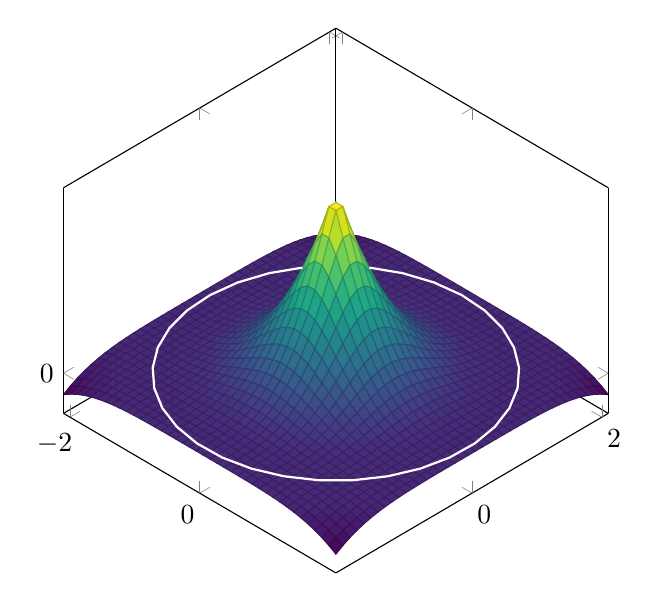
\begin{tikzpicture}
    \begin{axis}[
        view={45}{45},
        xtick={-2, 0},
        ytick={0, 2},
        ztick={0},
        domain=-2.1:2.1,
        domain y=-2.1:2.1,
        samples=40,
        samples y=40,
        colormap/viridis,
        width=8.5cm, height=8.5cm,
    ]
        \addplot3[surf] {0.25 / (pi * 1^3) * ((sqrt(x^2 + y^2) > 0.04) ? (2 - sqrt(x^2 + y^2))^3 : (sqrt(x^2 + y^2)^2 * (3 * sqrt(x^2 + y^2) - 6) + 4))};
        \addplot3[domain=-214.5:124.5, samples=32, samples y=0, thick, white] ({2*cos(x)}, {2*sin(x)}, {0});
    \end{axis}
\end{tikzpicture}

\medskip
The graph shows a~mass kernel function used to~compute boundary particle masses (more on~that later) and densities.
The~two horizontal axes represent the~relative position of~neighboring particles in~multiples of~the~smoothing radius, which is obtained as follows:

\[ \mathbf{r}'_j = \frac{|\mathbf{r}_i - \mathbf{r}_j|}{h} \]

Then, the~relative distance is computed as:

\[ d_j = \sqrt{\mathbf{r}'_j \cdot \mathbf{r}'_j} \]

The~SPH solver checks this distance and skips the~neighboring particle if its relative distance exceeds number two.
The~kernel graph depicts the~border between the~points with valid distance and the~points exceeding this threshold as~a~white circle.
In~other words, if the~distance between a~particle and its neighbor is greater than twice the~smoothing radius, the~neighbor is skipped and not considered.
The~kernel functions have a~characteristic shape.
There is the~peak in~the~middle, with~the~function falling off to~zero values at~distances equal to~two.
The~equation of~the~mass kernel function looks like this:

\[ W_m(d_j, h) = \frac{0.25}{\pi h^3} \cdot \begin{cases} (2 - d_j)^3, & d_j > 1, \\ d_j^2 \cdot (3d_j - 6) + 4, & d_j \leq 1 \end{cases} \]

\subsection*{Uniform Grid Neighbor Search}

The~SPH solver can sort particles to~a~uniform grid to~speed up neighbor search.
The~fundamental idea behind this approach is to~divide the~simulation space into a~grid of~uniform cells with~size equal to~the~smoothing radius, where each cell contains a~list of~the~particles located within its boundaries.
When a~particle evaluates its neighbors, it no longer needs to~perform a~naive search in~the~entire space.
Instead, the~algorithm only considers those particles within the~same cell and adjacent cells, significantly reducing the~number of~comparisons needed.
The~maximum distance of~two particles in~two adjacent cells cannot exceed twice the~size of~the~cell, i.e., twice the~smoothing radius.
This directly corresponds to~the~cut-off of~the~kernel functions.
The~uniform grid is rebuilt from scratch on~each simulation time step as~follows:

\begin{lstlisting}
// Map particles to cells
for p in particles
    cells_map[p] = CellIndex(p.position)
// Initialize cells lookup
fill(cells_lookup, 0)
for c in cells_map
    cells_lookup[c]++
exclusive_scan(cells_lookup)

// Sort particles by cell index
copy(cells_lookup, cells_copy)
for p in particles
    c = cells_map[p]
    i = cells_copy[c + 1]--
    i--
    sorted[i] = p
\end{lstlisting}

First, each particle is mapped to~a~cell index ranging from~zero to~the~total cell count.
Then, the~cell lookup is initialized.
Its size equals the~total cell count plus one and is initially set to~zero.
All the~cell indices of~particles are iterated, and each cell index in~the~cell lookup array is incremented by~one.
After the~exclusive scan, the~cell lookup contains a~growing sequence of~numbers starting from~zero and ending with the~total cell count.
These numbers will later be used as~offsets to~the~array of~particles.
The~cell lookup is copied to~a~temporary array, which is used to~sort particles.
When sorting, the cell index is obtained.
Then, this cell index is used to~look up~the~offset of~the~following cell index.
The~offset of~the~following cell index is decremented by one, meaning it no longer points to~the~first particle of~the~following cell but to~the~last particle of~the~current cell.
This offset is then used to~determine the~new position of~a~particle in~a~sorted array.
Iterating over the~following particles decreases the~original offset further, pointing to~new distinct locations where the~corresponding particles should be placed.
At~the~end of~the~sorting process, the~sorted array contains particles with~the~same cell index group together, and the~cell lookup array contains offsets to~the~first particle in~each cell list.

\begin{lstlisting}
for p in particles
    cell = CellPosition(p.position)

    // Check all adjacent cells
    for x in -1..1
    for y in -1..1
    for z in -1..1
        c = CellIndex(cell + (x, y, z))
        if c < 0 or c >= cell_count
            continue

        // Index of the first particle
        // of the current cell
        j = cells_lookup[c]

        // Check against index
        // of the first particle
        // of the following cell
        while j < cells_lookup[c + 1]
            // Do stuff
            j++
\end{lstlisting}

When searching for~neighbors, the~SPH checks all the~adjacent cells and extracts the~index of~the~first particle in~that cell from the~lookup array.
Then, it iterates through the~particles until it hits the~first particle in~the~following cell.

\subsection*{Boundaries}
Fluid particles must be contained within the~simulation space. Additionally, a~solid object within this space may interact with~the~fluid.
A~straightforward approach to~addressing the~boundary problem is to~reflect particles.
This involves adjusting the~velocity and position of~fluid particles when they come into~contact with~the~boundary, effectively bouncing them back into~the~fluid domain.
Another approach is to~use static boundary particles that simulate the~behavior of~solid surfaces.
These particles do not represent the~fluid, but they are included in~the~interpolation in~the~same manner as~fluid particles, thereby enforcing boundary conditions through their interaction with~the~fluid.
Most importantly, utilizing boundary particles increases the~visual appeal of~the~simulation.

The~placement of~boundary particles can be challenging for~complex shapes.
However, the~simulation space described in~this report is a~simple cube box.
In~this case, the~static boundary particles are distributed uniformly along the~box's walls.
The~distance between these particles is crucial.
While shorter distances enhance the~numerical stability of~the~simulation and help prevent artifacts, they also increase computation time, as~more particles need to~be processed.
Therefore, the~implementation positions the~boundary particles at~a~distance equal to~the~smoothing radius, which is a~good compromise.

\section*{Build and Run}
The~code is written in~C++17 and uses OpenMP and CUDA for~multi-core and many-core computation.
The~results of~the~deprecated MPI support for distributed processing are presented in~the~results section, but the~MPI code is not included as~it proved to~be very buggy.
On~UNIX platforms, the~meson build system is used to~compile the~project, while on~Windows, one needs to~compile the~project in~Visual Studio.
The~window system used is the~SDL2 library, and the~rendering is done via~OpenGL.

\subsection*{Compilation}
The~user can compile the meson project using the~included Makefile on~UNIX platforms by~simply running the~\texttt{make} command.
The~meson will download and compile the~necessary libraries, including the~SDL2.
However, the~compilation may fail on~some systems, including NixOS, so~the~user is advised to~install the~SDL2 package using his package manager of~choice.
The~compilation outputs the~\texttt{fluid} binary executable.
If~the~computer has a~discrete Nvidia GPU on~UNIX system enabled by~Nvidia Prime offloader, setting some environment variables before launching the~executable is necessary.
The~user can run the~\texttt{make run} command that sets the~variables and executes the~binary for~ease of~use.

\bigskip
On~Windows systems, the~compilation is more complicated.
The~attached Visual Studio solution includes the~project configuration, but it relies on~the~location of~header files in~the~\texttt{subprojects} folder used by~the~meson build system.
The~user is thus advised first to~run the meson build using the~commands \texttt{meson setup build} and \texttt{meson compile -C build}, which is expected to~fail, but it downloads the~corresponding headers.
Then, the~user can compile the~project from~within the~Visual Studio.

\bigskip
If~the~computer does not have a~CUDA-enabled GPU, the~user has to~delete the~\texttt{USE\_CUDA} definition, which serves as~a~compile-time configuration.
To~do so, the~user must comment out the~corresponding lines in~the~meson.build file.
The~comments in~the~file should aid the~user.
In~Visual Studio, the~user must delete the~definition from~the~project configuration by~right-clicking on~the~solution in~the~solution explorer.

\subsection*{Runtime Configuration}
The~behavior of~the~simulation can be altered through the~following configuration options:

\begin{lstlisting}
{
  "window": {
    "title": "Fluid",
    "width": 800,
    "height": 800,
    "point_size": 1.5
  },
  "compute": {
    "cli": false,
    "gpu": true,
    "gpu_threads": 256,
    "omp_threads": 8,
    "steps": -1
  },
  "simulation": {
    "delta": 0.0025,
    "space_size": 1.2,
    "smooth_radius": 0.04,
    "fluid_grid": [24, 32, 24],
    "box_boundary": false
  },
  "fluid": {
    "gravity": -9.8,
    "mass": 0.0000765,
    "density": 1.0,
    "viscosity": 0.05,
    "stiffness": 10.0
  }
}
\end{lstlisting}

The~\texttt{title}, \texttt{width}, and \texttt{height} options are self-evident.
The~\texttt{point\_size} option sets the~size of~the~fluid particle in~screen space.
\texttt{cli} toggles between graphical and terminal-only execution, but steps must be positive to~make it work.
\texttt{gpu} toggles between CPU and GPU computation.
\texttt{gpu\_threads} sets the number of~threads per~block.
It is advised to~use multiple of~the~size of~the~CUDA warp, i.e., 32.
Other values may result in~undefined behavior.
\texttt{omp\_threads} sets the~number of~threads to~use on~the~CPU.
The~\texttt{steps} represents a~number of~simulation steps after which the~execution should stop and print out the~computation time.
If~the value is set to~$-1$, the~simulation proceeds indefinitely unless paused or shut down.
\texttt{delta} is a~fixed simulation time step.
Large values result in~unstable simulation.
\texttt{space\_size} defines the~length of~a~side of~the~cube simulation space, while \texttt{smooth\_radius} defines the~cut-off distance of~smoothing kernel functions and the~length of~a~single cell in~the~cell grid.
Increasing this value results in~a~more correct approximation but significantly slower computation.
\texttt{fluid\_grid} defines the~initial configuration of~fluid particles.
texttt{box\_boundary} toggles between boundaries of~the~box using static boundary particles or not.
Then, five constants \texttt{gravity}, \texttt{mass}, \texttt{density}, \texttt{viscosity}, and \texttt{stiffness} defining the~properties of~the~fluid follow.

The~\texttt{config.json} file is open by~default if~the~executable is run without an~argument.
However, \texttt{configs} directory contains three configurations used in~the~benchmark results section.
Such a~configuration can be selected by~running the~executable as \texttt{./fluid configs/<1-3>.json}.

\subsection*{Controls}
Hold the~left mouse button and move with the~cursor to~rotate the~camera.
Scroll the~mouse wheel to~zoom in~and out.
The~space bar commences the~simulation while another press pauses it.
The~\texttt{R} key resets the~simulation to~its initial state.
The~\texttt{B} key shows or hides static boundary particles if such are configured.
Keys \texttt{1} to \texttt{4} change the~colorization of~the~fluid particles to~all blue, velocity-based, pressure-based, and density-based, respectively.
The~\texttt{F} key toggles between fullscreen and window.
Finally, the~escape closes the~application.

\section*{Implementation}
All of~the~codebase is located inside the~\texttt{source} folder.
The~\texttt{main.cpp}, \texttt{window.hpp}, \texttt{window.cpp}, \texttt{shader.hpp}, and \texttt{shader.cpp} are not particularly important in~discussing the~SPH solver.
A~quick reference in~the~form of~Doxygen documentation is available.

The~\texttt{particles.hpp} file defines a~structure of~particles.
The~structure points to~arrays of~various fluid properties like position, viscosity, or mass.
All these arrays are the~same length as~the~number of~particles.
However, the~cells lookup array is the~size of~the~total cell count plus one.
The~array stores offsets to~the~first particle in~each cell and is used in~neighbor search, as~previously discussed in~the~analysis section.
Note that there are two arrays for~positions and velocities.
Whenever particles are sorted to~cells, and the~cells lookup array is initialized, the~sorting of~positions and velocities does not happen in~place but rather to~the~other two arrays.
Those arrays are then marked as~the~current, and when the particles are sorted again, the positions and velocities are sorted from those arrays back to~the~former.
These swap buffers are utilized to~enable parallel sorting.

The~\texttt{fluid.hpp} defines the~actual fluid simulation structure.
The~data type holds many parameters required for~the~computation of~the~simulation.
The~curious reader is advised to~check Doxygen, but the~report will discuss the~inner workings in~the~upcoming text.

The~\texttt{fluid.cpp} file forwards function calls to~the~CPU or the~GPU implementation and is a~great place to~understand what is happening.
The~\texttt{Create} and \texttt{Destroy} functions create and destroy the~simulation, respectively.
The~JSON file is parsed, and the~configuration is loaded into~the~structure.
Then, the~\texttt{Reset} function is called, which resets the~simulation to~the~initial state by placing the~particles into~the~simulation space.
Additionally, if~static boundary particles are to~be used, they are placed in~the~space, sorted into~cells, and their masses are set.
When the~simulation commences, the~\texttt{Update} function is called, and it calculates one SPH solver simulation step.
The~actual implementation of~these functions is found in~\texttt{cpu.cpp} and \texttt{gpu.cpp} files.

\subsection*{OpenMP}
When the~compute on~the~CPU is requested, and the~\texttt{PlaceParticles} function is called, the~implementation dynamically allocates all the~arrays and initializes values.
Every property of~each particle is set to~zero, except the~mass, which is set to~the~mass constant.
The~\texttt{fluid\_grid} configuration parameter dictates the~initial fluid shape in~the~simulation space's center.
Static boundary particles are optionally placed along the~box's walls but inside the~simulation space, so~the~particle sorting into~cells works on~them.
The~\texttt{omp\_chunk} variable is set to~the~number of~fluid particles divided by~the~number of~OpenMP threads \texttt{omp\_threads}.

Sorting the~particles in~the~\texttt{SortParticles} function follows the~pseudocode presented in~the~analysis section of~the~report.
Practically any loop inside the~\texttt{cpu.cpp} file is prepended with~the~following OpenMP directives.
The~scheduling policy used for~iterations is static.
Each OpenMP thread is assigned a~chunk of~data of~size \texttt{omp\_chunk}:

\begin{lstlisting}
#pragma omp parallel for \
    num_threads(omp_threads) \
    schedule(static, omp_chunk)
\end{lstlisting}

Incrementing the~corresponding cell in~the~cells lookup array must be handled securely.
The~OpenMP directive ensures that the~following statement updates the~shared variable atomically, preventing race conditions:

\begin{lstlisting}
for (int i = 0; i < p.size; i++) {
    #pragma omp atomic update
    p.cells_lookup[cells_map[i]]++;
}
\end{lstlisting}

When sorting the~particles into~the~second swap buffer, the~copy of~the~cells lookup is decremented.
Again, such an~operation must be safe.
This time, a~directive with \texttt{capture} instead of~\texttt{update} is used to~capture the~decremented value into a~variable correctly.
The~variable has to~be declared before the~OpenMP directive to~make it work:

\begin{lstlisting}
for (int i = 0; i < p.size; i++) {
    int c = cells_map[i];
    int j;
    #pragma omp atomic capture
    j = p.cells_copy[c + 1]--;
    j--;

    // Place particle from index i to j
}
\end{lstlisting}

The~\texttt{Update} function is split into five additional function calls: \texttt{ApplyGravity}, \texttt{ApplyViscosity}, \texttt{ApplyDensity}, \texttt{ApplyPressure}, and \texttt{Integrate}.
These methods update the~particles' properties and then update each particle's velocity vector.
At~the~end of~the~\texttt{Update} function, all particles move to~their new position.

\subsection*{MPI}
In a~distributed multi-process environment, the~\texttt{SortParticles} function is challenging to~parallelize.
The~deprecated MPI implementation chose a~single driving process that handled the~sorting and distributed the~sorted arrays to~other processes.
The~driving process was chosen as~the~one with~the~MPI rank equal to~zero:

\begin{lstlisting}
int mpi_rank;
int mpi_size;
MPI_Init(NULL, NULL);
MPI_Comm_rank(MPI_COMM_WORLD, &mpi_rank);
MPI_Comm_size(MPI_COMM_WORLD, &mpi_size);
\end{lstlisting}

Now, during the~computation, each process checks against its rank.
If~it is not the~driving process, it waits for~the~one at~the~next \texttt{MPI\_Barrier} and then collects the~data broadcasted from~the~driving process to~all other processes:

\begin{lstlisting}
if (mpi_rank == 0)
    SortParticles(fluid);

MPI_Barrier(MPI_COMM_WORLD);
MPI_Bcast(fluid.cells_lookup,
    cell_count + 1, MPI_INT,
    0, MPI_COMM_WORLD);
MPI_Bcast(fluid.positions,
    fluid.size * sizeof(float3), MPI_BYTE,
    0, MPI_COMM_WORLD);
MPI_Scatter(fluid.velocities,
    chunk_size * sizeof(float3), MPI_BYTE,
    fluid.velocities + chunk_index,
    chunk_size * sizeof(float3), MPI_BYTE,
    0, MPI_COMM_WORLD);
\end{lstlisting}

The~positions of~all particles are broadcasted to~all the~processes since the~SPH solver computation requires all that information.
However, each velocity is only updated by~a~single process.
In~that case, the~driving process does not need to~send out the~whole velocities array to~all processes but instead distributes corresponding chunks of~data to~each using the~\texttt{MPI\_Scatter} function.
Some functions, like \texttt{ApplyPressure}, need all the~particles' values of some property, so~the~\texttt{MPI\_Allgather} function is used to~collect the~corresponding chunk of~data from~each of~the processes on~all of~the~processes.
Upon doing so, each process has a~complete copy of~the~corresponding property array:

\begin{lstlisting}
ApplyGravity();

MPI_Barrier(MPI_COMM_WORLD);
MPI_Allgather(/* velocities */);
ApplyViscosity();

MPI_Barrier(MPI_COMM_WORLD);
ApplyDensity();

MPI_Barrier(MPI_COMM_WORLD);
MPI_Allgather(fluid.densities +
    chunk_index, chunk_size,
    MPI_FLOAT, fluid.densities,
    chunk_size, MPI_FLOAT,
    MPI_COMM_WORLD);
ApplyPressure();

MPI_Barrier(MPI_COMM_WORLD);
MPI_Allgather(/* velocities */);
Integrate();
\end{lstlisting}

\subsection*{CUDA}
The~code related to~Nvidia's CUDA can be easily spotted since it is always between \texttt{USE\_CUDA} define guards.
Most of~the~relevant code is in~the~\texttt{gpu.cpp} file, but two other notable differences exist between the~CPU and GPU versions.
First, declaring the~fluid simulation structure in~the~\texttt{fluid.hpp} file introduces new variables related to~the~CUDA execution graphs.
Second, the~\texttt{Reset} function in~the~\texttt{fluid.cpp} also introduces a~new function call, \texttt{Setup}, which utilizes the~newly created variables and is implemented in~the~\texttt{gpu.cpp} file.
The~\texttt{Setup} function is only called once to~setup the~execution graphs before the~simulation:

\begin{lstlisting}
int blocks = (fluid.size + gpu_threads - 1) / gpu_threads;
cudaStreamCreate(&stream);

// Setup for each of the swap buffers
for (int i = 0; i < 2; i++) {
    cudaStreamBeginCapture(stream,
        cudaStreamCaptureModeGlobal);

    ApplyGravity_CUDA<<<blocks,
        gpu_threads, 0, stream>>>(
        /* args */);

    ApplyViscosity_CUDA<<<blocks,
        gpu_threads, 0, stream>>>(
        /* args */);

    AddViscosity_CUDA<<<blocks,
        gpu_threads, 0, stream>>>(
        /* args */);

    ApplyDensity_CUDA<<<blocks,
        gpu_threads, 0, stream>>>(
        /* args */);

    SetPressure_CUDA<<<blocks,
        gpu_threads, 0, stream>>>(
        /* args */);

    ApplyPressure_CUDA<<<blocks,
        gpu_threads, 0, stream>>>(
        /* args */);

    Integrate_CUDA<<<blocks,
        gpu_threads, 0, stream>>>(
        /* args */);

    cudaStreamEndCapture(stream, graph[i])
    cudaGraphInstantiate(&exec[i],
        graph[i], NULL, NULL, 0);
}
\end{lstlisting}

The~\texttt{Setup} function utilizes a~CUDA stream to~capture CUDA kernel calls within the~CUDA execution graph.
Once the~capture process concludes, the~graph is instantiated and ready for~future launches.
This procedure is repeated twice because the~implementation employs two swap buffers for~storing positions and velocities.
The~stream capture records the~addresses of~the~pointers; changing the~swap index is not enough.
As~a~result, two execution graphs are created and instantiated for one of~the~two sets of~swap buffers.

Additionally, there are new kernel functions called \texttt{AddViscosity} and \texttt{SetPressure}.
These functions are necessary because the \texttt{\_\_syncthreads()} directive, used within a~CUDA kernel, only synchronizes threads within the~same block.
The~solver, however, requires synchronization across all particles.
Unfortunately, using stream capturing with \texttt{cudaMemsetAsync} did not yield the~desired results, since \texttt{cudaMemset} only sets bytes, while larger data types, such as~floats, are needed.

With~the~instantiated CUDA execution graphs, the~captured sequence of~kernel calls is executed in~the~\texttt{Update} function as~follows:

\begin{lstlisting}
cudaGraphLaunch(exec[swap], stream);
cudaStreamSynchronize(stream);
\end{lstlisting}

\bigskip
Another function that is exclusive to~the~GPU implementation is the~\texttt{Draw} function.
Here, CUDA interoperability with OpenGL is utilized to~directly copy the~data from~the~CUDA buffer to~the~OpenGL's vertex buffer object:

\begin{lstlisting}
struct cudaGraphicsResource *resource;

glBindBuffer(GL_ARRAY_BUFFER, vbo);
glBufferData(GL_ARRAY_BUFFER,
    fluid.size * sizeof(float3),
    NULL, GL_DYNAMIC_DRAW);

cudaGraphicsGLRegisterBuffer(&resource,
    vbo, /* just too long flag */);
cudaGraphicsMapResources(1, &resource);

void *ptr;
size_t size;
cudaGraphicsResourceGetMappedPointer(
    &ptr, &size, resource);

cudaMemcpy(ptr, fluid.positions,
    fluid.size * sizeof(float3),
    cudaMemcpyDeviceToDevice);

glDrawArrays(GL_POINTS, 0, fluid.size);

cudaGraphicsUnmapResources(1, &resource);
\end{lstlisting}

The CUDA registers a~graphics resource that encapsulates the~OpenGL vertex buffer object.
Then, it maps the~resource into the~memory, and the~pointer is obtained.
\texttt{cudaMemcpy} copies data to~the~vertex buffer, and the~contents can be drawn.
Finally, the~CUDA graphics resource is unmapped.

\bigskip
The~OpenMP CPU version of~\texttt{SortParticles} uses atomic directives to~ensure correct and safe cell lookup and sorting initialization.
The~CUDA GPU function uses \texttt{atomicAdd} and \texttt{atomicSub} calls, achieving the~same.
Furthermore, since they operate on~the~global memory, the~atomicity works across all the~particles, not only in~the~context of~the~current block.

\bigskip
\section*{Results}
The~implementation is benchmarked on~three different CPUs: Intel Core i7-8565U mobile CPU with four cores, 1.8 GHz base, and 4.6 GHz maximum clock speed.
It boasts 8 megabytes of~cache and consumes 25 Watts.
The~following CPU is an~AMD Ryzen~5 5600X desktop-class CPU.
Its six cores run on~a~3.7 GHz base and 4.6 GHz maximum clock speed.
It requires 65 Watts and has 3 megabytes of~L2 and 32 megabytes of~L3 cache.
They both support hyperthreading.
The~last CPU is the~SOPHON SG2042, a~RISC-V processor with a~massive 64 cores in~16 clusters.
Each cluster shares a~1-megabyte L2 cache, and the~whole CPU uses a~64-megabyte system cache.
Its base frequency stands at~2~GHz.
The~CPU typically consumes 120 Watts.

The~discrete mobile GPU tested is Nvidia's GeForce MX250.
It has 384 shading units in~3~streaming multiprocessors.
It operates at~around 1520 MHz and drains 25 Watts.
On~the~contrary, the~powerful desktop-class Nvidia RTX 3070, with clock speeds of~1815 MHz, boasts 5888 CUDA cores.
It requires a~650-watt power supply.

\begin{figure}[h!]
    \centering
    \includegraphics[width=0.34\textwidth]{images/show1.png}
    \includegraphics[width=0.34\textwidth]{images/show2.png}
\end{figure}

The~RISC-V CPU in~the~Milk-V Pioneer desktop may be the~first 64-core RISC-V CPU that got to~run a~fluid simulation:

\begin{figure}[h!]
    \centering
    \includegraphics[width=0.5\textwidth]{images/riscv.png}
\end{figure}

The~configs directory contains three configuration files, named 1, 2, 3 in~the table below, that were used in~the~measuring for~the~following table.
The~first configuration simulates 5,632 fluid particles in~a~uniform grid of~15,625 cells.
The~second increases the~number of~particles to~i18,432 and number of~cells to~i27,000.
The~last configuration is the~most demanding, with~particles and cells equal to~49,152 and ~52,735, respectively.
Benchmark uses 1,500 simulation steps.
The~reported times are in~milliseconds.

\begin{table}[h!]
    \centering
    \begin{tabular}{|c||c|c|c|}
        \hline
        CPU & 1 & 2 & 3 \\
        \hline \hline
        i7-8565U & 10,211 & 39,555 & 173,139 \\
        5600X & 31,260 & 124,411 & - \\
        SG2042 & 23,459 & 23,115 & 48,472 \\
        \hline
        MX250 & 116,623 & - & - \\
        RTX 3070 & 5,974 & 14,725 & 36,475 \\
        \hline
    \end{tabular}
\end{table}

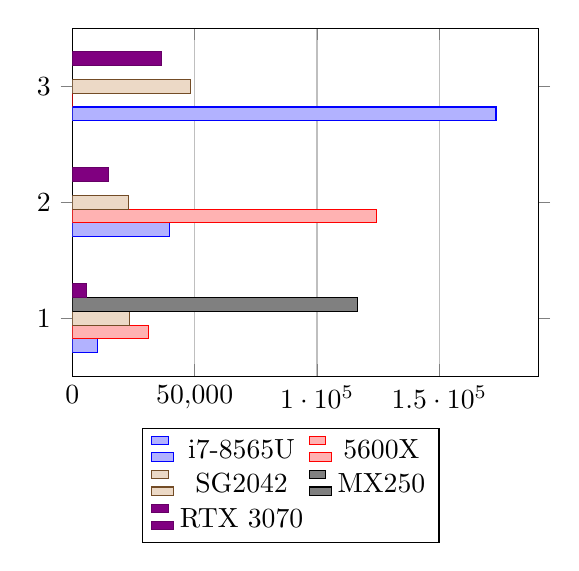
\begin{tikzpicture}
    \begin{axis}[
        xbar=0pt,
        bar width=5pt,
        enlarge y limits=0.25,
        width=7.5cm,
        height=6cm,
        legend style={at={(0.15,-0.15)}, anchor=north west, legend columns=2},
        symbolic y coords={1,2,3},
        ytick=data,
        xmin=0,
        scaled x ticks=false,
        xmajorgrids=true,
    ]
        \addplot coordinates {(10211,1) (39555,2) (173139,3)};
        \addplot coordinates {(31260,1) (124411,2) (0,3)};
        \addplot coordinates {(23459,1) (23115,2) (48472,3)};
        \addplot coordinates {(116623,1) (0,2) (0,3)};
        \addplot coordinates {(5974,1) (14725,2) (36475,3)};
        \legend{i7-8565U, 5600X, SG2042, MX250, RTX 3070}
    \end{axis}
\end{tikzpicture}

The~configurations used the~best settings for~each of~the~systems.
Intel CPU utilized 8 OpenMP threads, the~AMD CPU used 12, and the~SOPHON processor used 64.
Both GPUs ran on~256 threads per~block.
It is interesting to~see that the~mobile CPU on~Linux outperformed the~desktop CPU on~Windows machine by~such a~large margin.
The~Nvidia MX250 GPU ran quite well in~the~first hundreds of~iterations, but due to~the~power throttling, the~performance dropped significantly, and the~additional tests were not run.
Such a~drop is suspected to~be the~result of~the~underlying operating system, NixOS, driver support and power management.
Additionaly, the~MX250 GPU supports offloading via~Nvidia Optimus, a~feature which rarely works well on~Linux.
The following table shows the results of the same configuration but instead of 1,500 steps, the simulation prints out the computation time after 500 steps before the power throttling occurs.
Again, the times are in milliseconds.

\begin{table}[h!]
    \centering
    \begin{tabular}{|crr|}
        \hline
        MX250 & 500 steps & 1,500 steps \\
        \hline
        Total time: & 6,656.000 & 116,623.000 \\
        \hline
        Time per step: & 13.312 & 77.748 \\
        \hline
    \end{tabular}
\end{table}

Various runtime configuration options greatly influence the~simulation's performance, and the~following text discusses the~most important ones.
The~\texttt{omp\_threads} parameter is crucial for~the~OpenMP implementation, translating directly to~the~speedup.
The~following table shows the~speedup of~the~RISC-V CPU when the~number of~threads is increased.
The~speedup is proportional to~the~number of~threads as~expected on~1,500 simulation steps:

\begin{table}[h!]
    \centering
    \begin{tabular}{|cc|}
        \hline
        \texttt{omp\_threads} & \texttt{config1.json} \\
        \hline
        8 & 72,479 \\
        16 & 37,860 \\
        32 & 21,131 \\
        64 & 23,459 \\
        \hline \hline
        \texttt{omp\_threads} & \texttt{config2.json} \\
        \hline
        8 & 68,968 \\
        16 & 35,981 \\
        32 & 20,054 \\
        64 & 23,115 \\
        \hline
    \end{tabular}
\end{table}
\begin{table}[h!]
    \centering
    \begin{tabular}{|cc|}
        \hline
        \texttt{omp\_threads} & \texttt{config3.json} \\
        8 & 191,508 \\
        16 & 98,360 \\
        32 & 52,480 \\
        64 & 48,472 \\
        \hline
    \end{tabular}
\end{table}

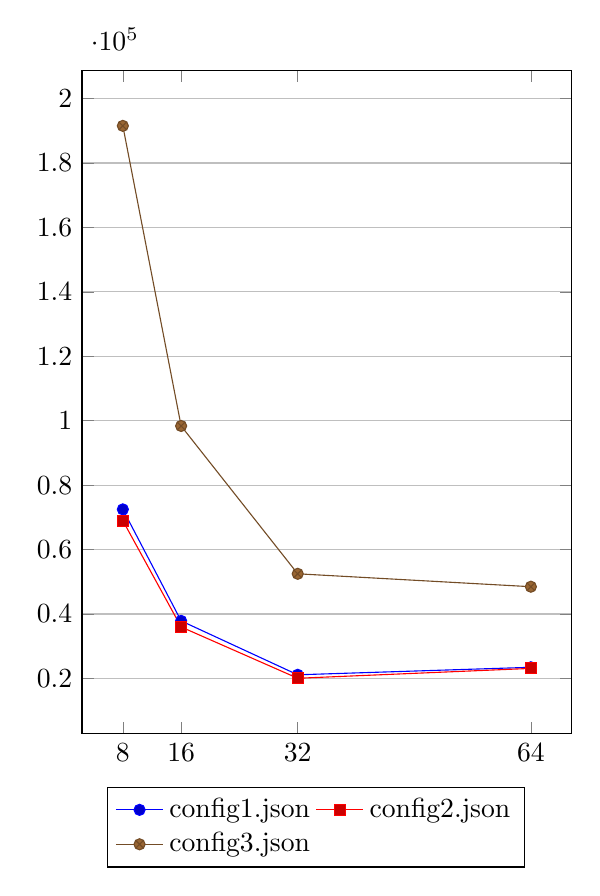
\begin{tikzpicture}
    \begin{axis}[
        width=7.8cm,
        height=10cm,
        legend style={at={(0.05,-0.08)}, anchor=north west, legend columns=2},
        xtick={8,16,32,64},
        ymajorgrids=true,
    ]
        \addplot coordinates {(8, 72479) (16, 37860) (32, 21131) (64, 23459)};
        \addplot coordinates {(8, 68968) (16, 35981) (32, 20054) (64, 23115)};
        \addplot coordinates {(8, 191508) (16, 98360) (32, 52480) (64, 48472)};
        \legend{config1.json, config2.json, config3.json}
    \end{axis}
\end{tikzpicture}

For~the~GPUs, the~\texttt{gpu\_threads} parameter does not play such a~significant role.
The~following table shows the~change in~speeds of~the~Nvidia RTX 3070 GPU when the~number of~threads per~block is changed on~1,500 simulation steps:

\begin{table}[h!]
    \centering
    \begin{tabular}{|cc|}
        \hline
        \texttt{gpu\_threads} & \texttt{config1.json} \\
        \hline
        64 & 3,714 \\
        128 & 3,781 \\
        256 & 5,974 \\
        512 & 11,237 \\
        \hline \hline
        \texttt{gpu\_threads} & \texttt{config2.json} \\
        \hline
        64 & 12,523 \\
        128 & 13,290 \\
        256 & 14,725 \\
        512 & 15,026 \\
        \hline \hline
        \texttt{gpu\_threads} & \texttt{config3.json} \\
        64 & 32,193 \\
        128 & 33,218 \\
        256 & 36,475 \\
        512 & 38,719 \\
        \hline
    \end{tabular}
\end{table}

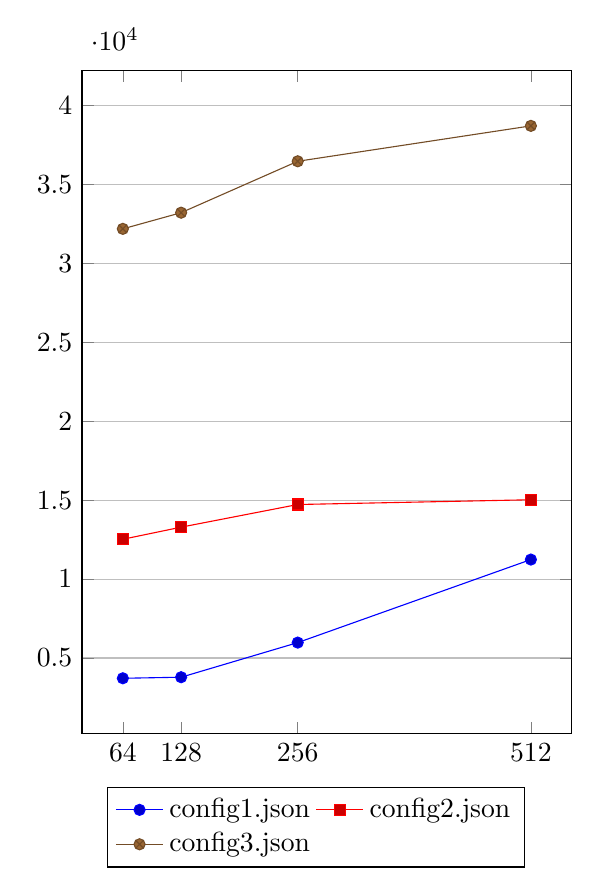
\begin{tikzpicture}
    \begin{axis}[
        width=7.8cm,
        height=10cm,
        legend style={at={(0.05,-0.08)}, anchor=north west, legend columns=2},
        xtick={64,128,256,512},
        ymajorgrids=true,
    ]
        \addplot coordinates {(64, 3714) (128, 3781) (256, 5974) (512, 11237)};
        \addplot coordinates {(64, 12523) (128, 13290) (256, 14725) (512, 15026)};
        \addplot coordinates {(64, 32193) (128, 33218) (256, 36475) (512, 38719)};
        \legend{config1.json, config2.json, config3.json}
    \end{axis}
\end{tikzpicture}

Another important parameter is the~\texttt{smooth\_radius}.
Increasing the~value results in~a~more accurate simulation but significantly slower computation.
Decreasing the~value speeds up the~simulation but may render the~simulation unstable.
The~following table presents the~impact of~various smoothing radii on~the~i7-8656U CPU on~the~second configuration on~750 simulation steps:

\begin{table}[h!]
    \centering
    \begin{tabular}{|cc|}
        \hline
        \texttt{smooth\_radius} & \texttt{config2.json} \\
        \hline
        0.02 & 4,333 \\
        0.03 & 8,716 \\
        0.04 & 17,990 \\
        0.06 & 39,899 \\
        0.08 & 79,939 \\
        \hline
    \end{tabular}
\end{table}
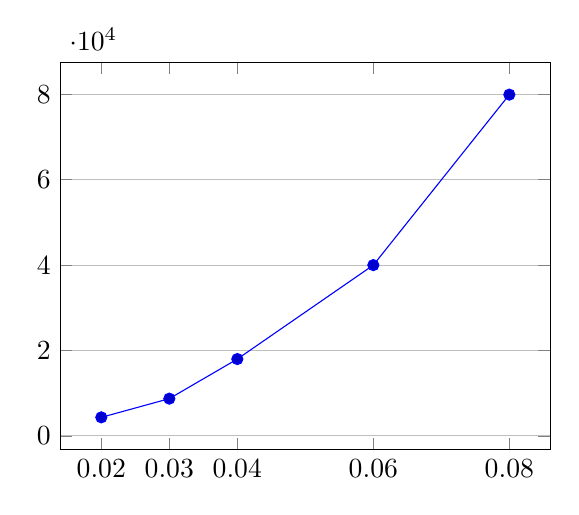
\begin{tikzpicture}
    \begin{axis}[
        width=7.8cm,
        height=6.5cm,
        xtick={0.02, 0.03, 0.04, 0.06, 0.08},
        ymajorgrids=true,
        scaled x ticks=false,
        xticklabel style={/pgf/number format/fixed}
    ]
        \addplot coordinates {(0.02, 4333) (0.03, 8716) (0.04, 17990) (0.06, 39999) (0.08, 79939)};
    \end{axis}
\end{tikzpicture}

The~following images show the~fluid simulation state after the~750 simulation steps with~the~smoothing radii of~0.02, 0.03, 0.04, and 0.08, respectively:

\begin{figure}[h!]
    \centering
    \includegraphics[width=0.185\textwidth]{images/radius2.png}
    \includegraphics[width=0.185\textwidth]{images/radius3.png}
    \includegraphics[width=0.185\textwidth]{images/radius4.png}
    \includegraphics[width=0.185\textwidth]{images/radius6.png}
\end{figure}

The~\texttt{box\_boundary} does not influence the~performance but alters the~simulation's visual appearance.
The~first image shows the~simulation without the~static boundary particles, while the~second image shows the~simulation with them:

\begin{figure}[h!]
    \centering
    \includegraphics[width=0.5\textwidth]{images/border.png}
    \includegraphics[width=0.5\textwidth]{images/no-border.png}
\end{figure}

The~invisible static boundary particles would look like this:

\begin{figure}[h!]
    \centering
    \includegraphics[width=0.45\textwidth]{images/boundary.png}
\end{figure}

When the~simulation is kept running until the~fluid settles, the~visual impact of~the~static boundary particles is even more apparent.
The~fluid without the~static boundary particles settled much faster and did not exhibit as~many eye-catching splashes as~the~one with the~static boundary particles.

Lastly, the~fluid simulation constants alter the~fluid's behavior.
Here are the~states of~the~fluid after 125 simulation steps with~the~viscosity set to~0.5, 0.4, 0.2, and 0.05, respectively.
The~0.5 viscosity results in~an~almost solid-like behavior, causing such pressures that the~fluid explodes:

\begin{figure}[h!]
    \centering
    \includegraphics[width=0.24\textwidth]{images/visc50.png}
    \includegraphics[width=0.24\textwidth]{images/visc40.png}
    \includegraphics[width=0.24\textwidth]{images/visc20.png}
    \includegraphics[width=0.24\textwidth]{images/visc5.png}
\end{figure}

\section*{Conclusion}
This report presented a~fluid simulation implementation using the~Smoothed Particle Hydrodynamics solver method both on~the~CPU and GPU.
The~resulting code was benchmarked on~various hardware configurations.
Real-time fluid simulation performance was achieved on~all tested systems with pleasing visual results.

\end{document}
